\chapter{فصل مقدمه} 
\pagenumbering{arabic}
\newpage
\section{مقدمه:}

در دو دهه گذشته پیشرفت های عظیمی صورت گرفته است که به طور موثری \gls{spintronic} و مغناطیس را ترکیب کرده است و به یک نیروی قدرتمند که حوزه دستگاه های حافظه را شکل می دهد، تبدیل شده است. مواد و پدیده‌های جدید با سرعت چشمگیری کشف می‌شوند و مجموعه‌ای رو به افزایش از \gls{building block} را فراهم می‌کنند که می‌توانند در طراحی \gls{Functional Device} ترانزیستور مانند آینده مورد استفاده قرار گیرند.

شروع تحولات دو دهه‌ی اخیر برای ترکیب \gls{spintronic} و مغناطیس از 
اثر مقاومت مغناطیسی بزرگ \gls{GMR} بود، این زمینه با اکتشافات جدید مانند اثر مقاومت مغناطیسی تونلی \gls{TMR}، انتقال گشتاور اسپینی \gls{STT} و اخیراً، پدیده های مدار اسپینی بالا از جمله اثر هال اسپینی بزرگ \gls{GSHE} و عایق های توپولوژیکی \gls{TI}.
دستگاه های حافظه \gls{spintronic} مبتنی بر \gls{TMR} و \gls{STT} قبلاً تجاری شده اند در حالی که دستگاه های منطقی \gls{spintronic} هنوز به طور فعال در حال بررسی هستند. مواد و پدیده های جدید با سرعت چشمگیری کشف می شوند که می توانند به عنوان مجموعه ای از "\gls{building block}" به طور مداوم در حال گسترش برای \gls{Functional Device} پیچیده در نظر گرفته شوند.

\section{تئوری انتقال الکترونی و اسپینی در مواد دو بعدی:}
در این فصل، مفاهیم مورد نیاز برای درک ترابرد الکترونی و اسپین در مواد دو بعدی جدا شده از\gls{bulk} ارائه می‌شود.
با مقدمه‌ای کوتاه بر اصل کار یک ترانزیستور اثر میدانی دنبال می شود. سپس، مفهوم تزریق اسپین در مواد غیر مغناطیسی مانند \gls{Graphene} نیز همراه با توضیح مختصری در مورد مدل دو کاناله برای انتقال اسپین در یک \gls{spin valve} معمولی توضیح داده شده است. همچنین، مسائل مربوط به \gls{conductivity mismatch} و \gls{relaxation} اسپینی ناشی از اتصالها مورد بررسی قرار می گیرد. 
% متعاقباً، انتقال اسپین در \gls{Graphene}، از جمله مفاهیم معادله انتشار اسپین، اندازه‌گیری دریچه اسپین ناجایگزیده و اندازه‌گیری تقدم اسپین \lr{Hanle} شرح داده می‌شود. بعداً، مکانیسم‌های مختلف \لمس{spin relaxation} برای انتقال اسپین در \gls{Graphene} معرفی شدند. در نهایت، مروری بر مطالعات نظری و تجربی در مورد انتقال اسپین در \gls{Graphene} تک و دو لایه، در مجاورت با \lr{TMD}، ارائه شده است.

\subsection{ترابرد الکترونی در مواد دو‌بعدی:}
در چهار دهه گذشته، مطالعات دقیقی برای درک انتقال بار الکترونی در نیمه هادی‌های لایه‌ای \gls{bulk}  انجام شده است.
ساختار نوار الکترونی یک نیمه هادی لایه‌ای \gls{bulk} بسته به برهمکنش بین لایه‌ای بین لایه‌های دو بعدی آن تغییر می‌کند و این امر به طور قابل توجهی بر ترابرد الکترونی تأثیر می‌گذارد. علاوه بر این، در چنین نیمه‌رسانای لایه‌ای \gls{bulk}، می‌توان ویژگی‌های مختلف انتقال بار (ناهمسانگردی) را برای جهت‌های درون صفحه \lr{(x-y)} و خارج از صفحه \lr{(z)} انتظار داشت. در اینجا، جهت \lr{x-y} مربوط به انتقال بار در طول و عرض مواد دو بعدی\gls{bulk} است، در حالی که جهت \lr{z} در امتداد ضخامت آن است. همچنین، با راه‌اندازی الکترواستاتیکی چنین مواد دو‌بعدی از طریق \gls{capacitive coupling}، می‌توان انتظار انباشتگی بالاتر حامل‌های بار در سطحی که نزدیک‌تر به \gls{gate} است، در مقایسه با تخلیه \gls{bulk} به دلیل غربالگری بار بود.

اخیراً، مواد دو بعدی جدا شده از گرافیت \gls{bulk}،\gls{Graphene}، توسط \gls{Novoselov} و همکاران\cite{novoselov2004electric} به دست آمده است. با این حال، \gls{Graphene} فاقد گاف نواری در ساختار نوار الکترونی خود است که برای \gls{realisation} \gls{FET} ای مبتنی بر منطق ضروری است. این منجر به جستجوی دسته جدیدی از مواد دو‌بعدی شده است که نیمه رسانا هستند، مانند فسفر سیاه\cite{li2014black}، \ce{MoS}\cite{radisavljevic2011single}، \gls{germanane}\cite{madhushankar2017electronic} و موارد دیگر. با انبوهی از مواد دوبعدی موجود که ویژگی‌های الکتریکی مختلف را ارائه می‌کنند، مطالعه انتقال بار الکترونی در نیمه‌رساناهای دو‌بعدی جدا شده \gls{bulk} افزایش یافته است. این علاقه زیاد به نیمه هادی های دو بعدی جدا شده \gls{bulk} عمدتاً به دلیل کاهش \gls{screening of charge carriers} در مقایسه با نیمه هادی‌های \gls{bulk} و به دلیل محصور شدن کوانتومی بیشتر حامل های بار به دلیل دو بعدی بودن آنها است.

\begin{figure*}[!ht]
    \centering
    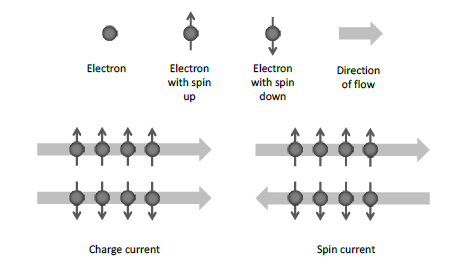
\includegraphics[width=0.9\linewidth]{spinchargecurent.png}
    \caption{برای یک جریان بار، الکترون های "بالا" و "پایین" در یک جهت جریان می یابند در حالی که برای یک جریان اسپین، الکترون های "بالا" و "پایین" در جهت مخالف جریان می یابند.}
    \label{fig:spinchargecurent}
\end{figure*}

\subsection{جریان بار و اسپین:}
الکترون یک ذره بنیادی یک اتم است که به دور هسته تشکیل شده از پروتون و نوترون می چرخد. بار الکتریکی یک الکترون منفی است و از مرتبه $1.602\times 10^{-19}$ کولن است. الکترون همچنین دارای یک تکانه زاویه‌ای ذاتی است که اسپین نامیده می شود که مقدار آن $\pm\frac{1}{2}$ است بسته به این که: اگر اسپین الکترون در جهت عقربه های ساعت/بالا باشد (+) یا خلاف جهت عقربه های ساعت/پایین (-). زمانی گفته می‌شود که جریان بار در سیستمی جریان دارد که الکترون‌ها، هر دو با اسپین بالا و پایین، در یک جهت جریان داشته باشند که در شکل\ref{fig:spinchargecurent} نشان داده شده است. چگالی کل جریان بار ($j$) فقط حاصل‌جمع سهم کل چگالی جریان اسپین بالا ($j_{\uparrow}$) و پایین ($j_{\downarrow}$) 
است، یعنی
\begin{equation}
    \vec{J}={\vec{J}}_{\uparrow }+{\vec{J}}_{\downarrow}
\end{equation}
در حالی که جریان اسپین از جریان اسپین بالا و پایین الکترون‌ها در جهت مخالف، همانطور که در شکل\ref{fig:spinchargecurent} نشان داده شده است، حاصل می‌شود. چگالی کل جریان اسپین ($j_s$) فقط تفاوت بین چگالی جریان اسپین بالا ($jـ\uparrow$) و پایین ($jـ\downarrow$) است، یعنی
\begin{equation}
    \vec{J}_{s} = \vec{J}_{\uparrow} - \vec{J}_{\downarrow}
\end{equation}
در حالی که \gls{Polarization} جریان اسپینی ($P_j$)،
\begin{equation}
    P_j = \frac{\vec{J}_{\uparrow} - \vec{J}_{\downarrow}}{\vec{J}_{\uparrow} + \vec{J}_{\downarrow}}
\end{equation}
\begin{figure*}[!ht]
    \centering
    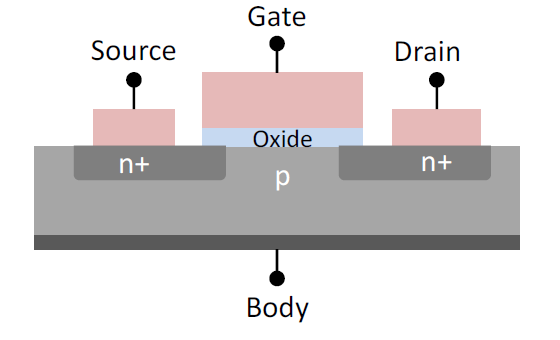
\includegraphics[width= 0.8\linewidth]{MOSFET.png}
    \caption{نمای مقطعی یک ماسفت که گیت، بدنه، منبع و پایانه تخلیه را نشان می‌دهد. گیت به صورت خازنی توسط یک لایه اکسید دی الکتریک نازک به کانال نیمه هادی جفت شده‌است.}
    \label{fig:mosfet}
\end{figure*}
\section{ترانزیستور اثر میدانی فلز-اکسید-نیمه هادی:}
ترانزیستور اثر میدانی فلز-اکسید-نیمه هادی(\gls{MOSFET}) نوعی ترانزیستور اثر میدانی (\gls{FET}) است. همانطور که در شماتیک دستگاه شکل \ref{fig:mosfet} نشان داده شده است، این یک دستگاه سه ترمینالی است که از الکترودهای \gls{gate}، \gls{source} و \gls{drain} تشکیل شده است. یک ماسفت معمولی شامل یک نیمه هادی است که بین یک جفت الکترود فلزی به نام \gls{source} و \gls{drain} متصل است. رسانایی نیمه هادی به طور خازنی توسط یک \gls{gate} فلزی تعدیل می‌شود که از طریق یک لایه اکسید نازک به کانال نیمه هادی متصل می‌شود، همانطور که در شکل \ref{fig:mosfet} نشان داده شده است. معمولا به صورت الکتریکی به زمین متصل می شود. ماسفت‌ها بسته به نوع حامل های بار در کانال نیمه هادی طبقه بندی می‌شوند، یعنی به عنوان نوع \lr{n} یا \lr{p} مربوط به انتقال بار الکترون یا حفره در کانال.
ترانزیستور نشان داده شده در شکل \ref{fig:mosfet} یک ماسفت سیلیکونی نوع \lr{n} است که در آن نیمه هادی سیلیکونی \gls{doped} شده با حفره است. سیلیکون با \gls{doped} بسیار الکترونی \lr{(n+)} به عنوان \gls{source} و الکترودهای \gls{drain} استفاده می شود. \gls{gate} معمولاً از \gls{polysilicon} تشکیل شده است که مانع اکسید آن \gls{silicon-di-oxide} است. کاربرد اصلی ماسفت استفاده از آن به عنوان یک کلید منطقی است که با روشن-خاموش کردن (که در منطق دیجیتال به صورت 1(0) نمایش داده می شود) جریان جاری در کانال نیمه هادی محقق می شود. برخی از عواملی که یک ماسفت خوب را مشخص می کند، \gls{operational voltage} آن، سرعتی که می توان جریان را روشن و خاموش کرد و ابعاد ترانزیستور است. ماسفت‌ها به طور مداوم برای دستیابی به عملکرد بهتر با مهندسی مواد و ابعاد کانال نیمه هادی، منبع، تخلیه و گیت در حال توسعه هستند.

\subsection{ترانزیستورهای اثر-میدانی گرافینی:}

% \gls{Graphene} اولین ماده دوبعدی کشف شده است [1]. کشف خصوصیات حیرت انگیز \gls{Graphene} مجموعه ای از مواد جدید را به وجود آورده است که به عنوان "مواد دو بعدی" شناخته می شوند [2-4]. فرم های دو بعدی برای بسیاری از کاربردها یک منطقه نسبتاً هیجان انگیز و جدید است [5 ، 6]. معمولاً مواد دو بعدی دارای بسیاری از خصوصیات فیزیکی برجسته هستند که برای دستگاه های الکترونی ، مهندسی نانو ، تبدیل انرژی و فوتونیک امیدوار کننده است [7-11]. با توسعه سریع \gls{Graphene} ، اخیراً مواد دو بعدی ، مانند فسفرن ، 
% \lr{BN} ، ژرمن ، آنتیمونن ، سیلیسن ، آرسنن و دی الكوژنیدهای فلزات انتقالی ، مورد توجه گسترده قرار گرفته اند.

% توده ای از مواد با ضخامت اتم از نظر تئوری پیش بینی یا سنتز شده است [12–16]. با کمال تعجب ، آنها ساختارهای متفاوتی از \gls{Graphene} دارند ، این اختلاف از درجه های متفاوت خمیدگی حاصل می‌شود [17]. علاوه بر مواد دو بعدی لایه برداری شده از نمونه های بالک، برخی از مواد دوبعدی نیز می توانند از مواد بالک بدون فرم لایه ای تولید شوند ، مانند ترکیب بور تخت دوبعدی  \lr{GaN 2D} و هافنن [18 ، 19].

\begin{figure*}[!ht]
    \centering
    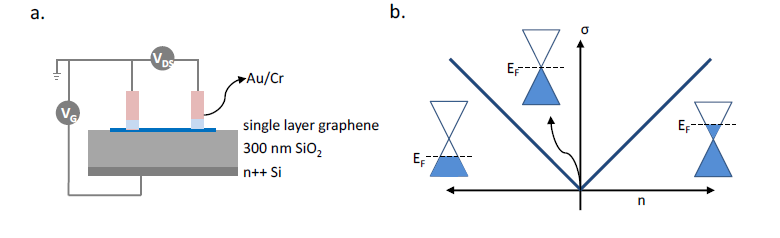
\includegraphics[width=\linewidth]{GrapheneFET.png}
    \caption{(الف). طرح‌واره دستگاه یک \lr{FET} با کانال گرافین بین الکترودهای منبع و تخلیه و یک گیت پشتی. (ب). طرحی از رسانندگی حامل بار ($\sigma$) گرافین \lr{FET} که تابعی از چگالی حامل بار \lr{(n)} ترسیم شده است. نمودار درونی – نواری گرافین با انرژی فرمی، $E_F$.}
    \label{fig:graphenefet}
\end{figure*}
تلاش دائمی در گسترش اثر میدان الکتریکی به فلزات صورت گرفته است. با این حال، این نیاز به فیلم‌های فلزی نازک اتمی دارد، زیرا میدان الکتریکی در فواصل کوتاه ($\le1\;nm$) برای فلزات \gls{bulk} غربال می‌شود. علاوه بر این، غلظت حامل بار در یک فلز \gls{bulk} در مقایسه با بارهای سطحی که می تواند توسط میدان الکتریکی القا شود، زیاد است. اولین تلاش برای تحقق بخشیدن به اثر میدانی در یک لایه اتمی از \gls{Graphene} نیمه فلزی توسط \gls{Novoselov} و همکاران\cite{novoselov2004electric} انجام شد که در آن، \gls{FET} \gls{Graphene} ساخته و مشخص شد و طرح‌واره دستگاه آن در شکل \ref{fig:graphenefet} نشان داده شده است. اعمال ولتاژ گیت \lr{($V_G$)} چگالی حامل بار \lr{(n)} و نوع حامل بار در \gls{Graphene} را تغییر می دهد، همراه با تغییر موقعیت انرژی فرمی، می‌توان چگالی حامل بار القایی را با اندازه‌گیری جریان (\lr{$I_{DS}$}) بین الکترودهای منبع و تخلیه را با جارو کردن ولتاژ (\lr{$V_{DS}$}) اعمال شده در سراسر الکترودهای تخلیه و منبع اندازه‌گیری کرد. رسانندگی اندازه گیری شده ($\sigma$)،$\sigma = I_{SD}/V_{SD}$، به عنوان تغییر در چگالی حامل بار همانطور که در شکل \ref{fig:graphenefet}(ب) نشان داده شده است، رسم شده است. محور مثبت \lr{n} مربوط به چگالی حامل الکترون ($E_F$ در نوار رسانایی) و محور منفی \lr{n} مربوط به چگالی حامل سوراخ ($E_F$ در باند ظرفیت) است. در حالی که در صفر است، از نظر تئوری انتظار می رود که چگالی حامل بار ($E_F$ در نقطه دیراک) در \gls{Graphene} نداشته باشد. تغییر رسانایی از فرمول \gls{Drude} پیروی می کند \cite{novoselov2004electric}، $\sigma = ne\mu$ (که \lr{e} بار الکترون است و $\mu$ تحرک حامل بار است). در نتیجه، تغییر خطی در $\sigma$ به عنوان تابعی از تغییر در n وجود دارد، همانطور که در شکل\ref{fig:graphenefet}(ب) نشان داده شده است. \gls{Novoselov} و همکاران \cite{novoselov2004electric} مقادیر معمول $\mu \approx 10000 cm^2/V·s$ و $n \approx 5 \times 10^{12} cm^{-2}$ را برای \gls{FET} های \gls{Graphene}ی خود اندازه گرفتند.
\begin{figure*}[!ht]
    \centering
    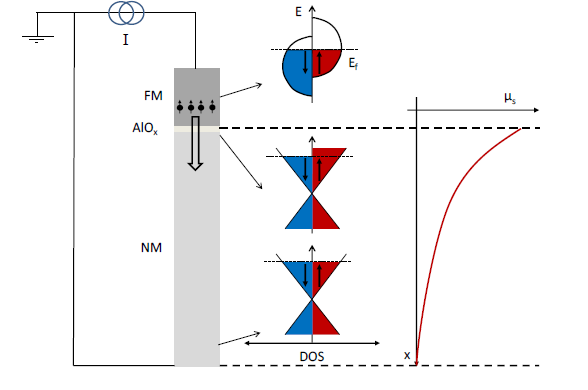
\includegraphics[width=\linewidth]{spininjection.png}
    \caption{تزریق اسپین از یک فرومغناطیس \lr{(FM)} به یک غیر آهنربا \lr{(NM)} همانطور که در قسمت سمت چپ شکل نشان داده شده است. پتانسیل شیمیایی اسپین در \lr{FM}، رابط )بین \lr{FM-\ce{AlOx}} و (\lr{NM}، و بخش عمده \lr{NM} در مرکز نشان داده شده است. فروپاشی نمایی انباشت اسپین القایی از رابط به بخش عمده \lr{NM} در قسمت سمت راست شکل نشان داده شده است.}
    \label{fig:spininjection}
\end{figure*}
\subsection{تزریق اسپین به مواد غیر مغناطیسی:}
در این بخش، فرآیند تزریق اسپینی از فرومغناطیس به غیر آهنربا به اختصار توضیح داده شده است. بعداً، مدل دو کاناله برای انتقال اسپین در یک \gls{spin valve} معمولی توضیح داده شده است. در نهایت، موضوع عدم تطابق رسانایی و \gls{relaxation} اسپینی ناشی از اتصالها مورد بررسی قرار می‌گیرد.
می توان با استفاده از فرومغناطیس (\gls{FM}) که دارای قطبش اسپین خالص است، به یک غیر آهنربا (\gls{NM}) مانند \gls{Graphene} تزریق اسپین انجام داد. همانطور که در شکل \ref{fig:spininjection}نشان داده شده است، در یک فرومغناطیس، عدم تعادل در چگالی حالات برای الکترون های اسپین بالا و پایین در انرژی فرمی وجود دارد. این عدم تعادل منجر به تفاوت در رسانایی برای کانال های اسپین بالا و پایین می شود. برای یک سیستم انتشار، هدایت برای هر کانال اسپین، $\sigma_{\uparrow(\downarrow)}$ را می توان به صورت زیر محاسبه کرد:
\begin{equation}
    \sigma_{\uparrow(\downarrow)} = g _{\uparrow(\downarrow)}(E_f) e^2 D_{\uparrow(\downarrow)}
    \label{eq:spintransport}
\end{equation}
که در آن، $g_{\uparrow(\downarrow)}$ چگالی حالات در انرژی فرمی $E_f$ و $D_{\uparrow(\downarrow)}$ میزان انتشار هر کانال اسپین است. $D_{\uparrow(\downarrow)}$ به این صورت تعریف می شود،
\begin{equation}
    D_{\uparrow(\downarrow)}=\frac{v_{f\uparrow(\downarrow)}I_{mfp\uparrow(\downarrow)}}{3}
\end{equation}
، که در آن $v_{F\uparrow(\downarrow)}$ سرعت فرمی، $l_{mfp\uparrow(\downarrow)}$ میانگین طول مسیر آزاد و ضریب $\frac{1}{3}$ ابعاد یک سیستم سه بعدی را محاسبه می کند.
هنگامی که جریان از \gls{FM} به \gls{NM} جریان می یابد، عدم تعادل اسپین خالص \gls{FM} به \gls{NM} در فصل مشترک القا می شود که منجر به یک حالت غیر تعادلی در \gls{NM} می شود. عدم تعادل اسپین ناشی از تجمع اسپین ($\mu_s$) نامیده می شود. $\mu_s$ به عنوان اختلاف پتانسیل شیمیایی اسپین برای کانال‌های اسپین‌آپ ($\mu_{\uparrow}$) و کانال‌های اسپین پایین ($\mu_{\downarrow}$) اندازه‌گیری می‌شود.$\mu_s=\frac{\mu{\uparrow}-\mu_{\downarrow}}{2}$.

علاوه بر این، هیچ عدم تعادل اسپینی در بخش \gls{bulk} \gls{NM} وجود ندارد، که منجر به انتشار اسپین‌ها از رابط به قسمت \gls{bulk} \gls{NM} می شود. همانطور که اسپین‌ها پخش می شوند، به دلیل برهم‌کنش آنها با ناخالصی‌ها یا فونون‌ها در بخش \gls{bulk} \gls{NM}، تحت پراکندگی قرار می گیرند. از این رو، آنها   تحت\gls{relaxation} قرار می گیرند. طول انتشار اسپین، $\lambda_s$ فاصله مشخصه ای است که در آن $\mu_s$ میرا می‌شود. $\lambda_s$ و $\mu_s$ به صورت، $\mu_s = \alpha\exp^{-x\lambda_s}$ مرتبط هستند. $\lambda_s$ زمان مربوط به \gls{relaxation} اسپین $\tau_s$ به عنوان $\lambda_s=\sqrt{D_s\tau_s}$ است، که در آن $D_s$ ضریب انتشار اسپین است. در مورد \gls{Graphene}، جایی که برهمکنش الکترون-الکترون مکانیسم پراکندگی غالب است، $D_s=D_c$، جایی که $D_c$ ضریب انتشار بار است. می توان قطبش اسپین جریان ($P_{j}^{NM}$) \gls{NM} را به صورت $P_{j}^{NM} = \frac{\mu_s}{j^{NM}R^{NM}}$ نوشت، که در آن $j^{NM}$ چگالی جریان بار در \gls{NM} و $R^{NM}$ مقاومت موثر \gls{NM} است.
می توان هندسه دستگاه را در شکل \ref{fig:twochannelmodel} با قرار دادن یک لایه نازک \gls{FM} ساخت. مانند \ce{Co}، با ضخامت حدود 60 نانومتر و با نسبت طول به عرض  10 نانومتر. بالای \gls{Graphene} یک لایه نازک اکسید از \gls{Aluminium oxide} به عنوان یک مانع تونلی بین \gls{FM} و \gls{Graphene} از برگشت اسپین‌های تزریق شده از \gls{Graphene} به \gls{FM} جلوگیری می کند.
\begin{figure*}[!ht]
    \centering
    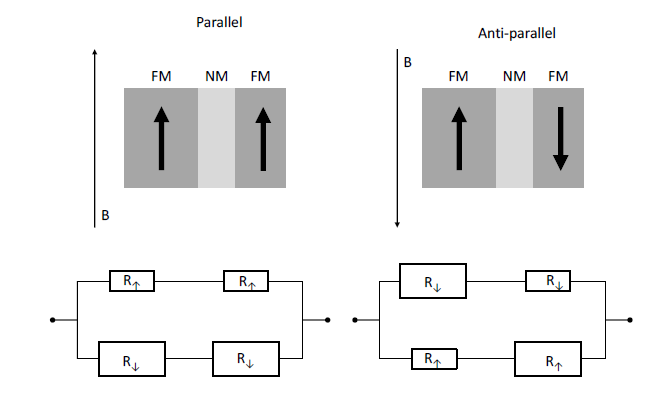
\includegraphics[width=\linewidth]{twochannelmodel.png}
    \caption{یک شیر اسپینی دو ترمینالی در شکل بالا با یک جفت \lr{FM} که یک \lr{NM} را ساندویچ می کند نشان داده شده است. شکل پایین مدل دو کاناله مربوطه را برای کانال اسپین بالا و پایین برای یک شیر اسپین دو ترمینالی نشان می دهد.}
    \label{fig:twochannelmodel}
\end{figure*}
\subsection{مدل دو کاناله:}
همانطور که در شکل\ref{fig:twochannelmodel}نشان داده شده است، یک غیر آهنربا \gls{NM} بین یک جفت فرومغناطیس \gls{FM} قرار می گیرد تا یک شیر اسپینی دو ترمینالی را تشکیل دهد. رسانایی برای الکترون های اسپین بالا و اسپین پایین در یک \gls{FM} همانطور که در رابطه \ref{eq:spintransport} نشان داده شده است متفاوت است و بنابراین رسانایی کل \gls{FM} $\sigma=\sigma_{\uparrow}+\sigma_{\downarrow}$ است، که $\sigma_{\downarrow}$ و $\sigma_{\uparrow}$ به ترتیب رسانایی برای اسپین بالا و پایین  هستند.

همانطور که در مدل مقاومت در شکل \ref{fig:twochannelmodel} نشان داده شده است، مقاومت برای کانال های اسپین بالا و پایین \gls{spin valve} دو ترمینالی به عنوان یک مدل دو کاناله نشان داده شده است. یک میدان مغناطیسی خارجی برای مغناطیسی کردن \gls{FM} در پیکربندی موازی اعمال می‌شود (فلش‌های شکل نشان‌دهنده جهت خالص مغناطیسی \gls{FM} هستند). در این هندسه، هنگامی که جریان از \gls{FM} چپ به \gls{FM} راست از طریق \gls{NM} می‌گذرد (مقاومت \gls{NM} نادیده گرفته می‌شود زیرا مستقل از اسپین است)، کانال اسپین‌بالا مقاومت پایینی را تجربه می‌کند در حالی که کانال اسپین پایین مقاومت بالایی را تجربه می‌کند. با این حال، \gls{switching} جهت مغناطیسی یکی از الکترودهای \gls{FM} از حالت بالا به پایین منجر به یک حالت پاد‌موازی می شود. در نتیجه، کانال‌های اسپین‌بالا و اسپین‌پایین یک مقاومت بالا و پایین را به صورت سری تجربه می‌کنند که در مدل مقاومت شکل \ref{fig:twochannelmodel}نشان داده شده است. بنابراین، مقاومت موثر برای الکترون‌های اسپین بالا در پیکربندی موازی کمتر از مقاومت در حالت پاد‌موازی است. در اصل، یک جریان قطبی اسپین از طریق\gls{spin valve} در پیکربندی موازی وجود دارد، در حالی که یک انباشته خالص اسپین برای پیکربندی پاد‌موازی ایجاد می‌شود که به صورت افت ولتاژ در سراسر \gls{spin valve} ظاهر می‌شود.

\subsection{عدم تطابق رسانایی و واهلش اسپینی ناشی از اتصال:}
تا اینجا، تزریق اسپین از یک \gls{FM} به یک \gls{NM} مورد بحث قرار گرفته است. با این حال، این تزریق اسپین می تواند به طور قابل توجهی تحت تاثیر عدم تطابق در رسانندگی اسپین برای یک \gls{FM} در یک \gls{NM} باشد. قبل از پرداختن به مشکل عدم تطابق رسانایی، باید مفهوم مقاومت اسپینی را ($R_s$) را درک کرد.
\begin{equation}
    R_{s}=\frac{\rho\lambda_{s}}{A}
\end{equation}
مقاومت اسپینی $R_s$، مقاومتی است که یک ماده برای جریان اسپین در آن ایجاد می کند. $\rho$ مقاومت، $\lambda_s$ طول انتشار اسپین و $A$ سطح مقطع ماده است. در مورد تزریق اسپین از یک \gls{FM} به یک \gls{NM}، مقاومت اسپین برای \gls{FM} ($R_{FM}$) کمتر از \gls{NM} ($R_{NM})$ است. منجر به جریان برگشتی اسپین‌ها به \gls{FM} می شود که در نهایت در \gls{FM} به تعادل می رسد زیرا طول عمر اسپین‌ها در \gls{FM} کوتاه است. این جریان برگشتی اسپین‌ها از \gls{NM} به \gls{FM} به دلیل مشکل عدم تطابق رسانایی است.
می توان مشکل عدم تطابق رسانایی را با قرار دادن یک مانع رابط مقاومتی بالا بین \gls{FM} و \gls{NM} حل کرد. سد رابط از اکسیدهای فلزی مانند \ce{Al2O3}، \ce{TiO2} و \ce{MgO} تشکیل شده است. مقاومت مرتبط با مانع رابط \ce{Rb}، بالاتر از مقاومت \lr{NM} است. و علاوه بر این، \ce{Rb} به عنوان تابعی از ضخامت مانع قابل تنظیم است.

\section{بوروفین:}
تحقیقات در مورد بور در ترکیبات مختلف را می توان به چند صد سال پیش بازگرداند ، زیرا بور دارای خاصیت فوق العاده‌ای است که می‌تواند تقریباً با تمام عناصر دیگر ترکیب شود. در میان آنها ، نیترید بور شش ضلعی \gls{h-BN} یک ترکیب بند وسیع \lr{III-V} است. این یک ماده لایه ای با ساختار گرافیت مانند است که در آن شبکه های مسطح شش ضلعی \gls{h-BN} مرتباً روی هم انباشته می شوند. \gls{h-BN} دارای پایداری شیمیایی بالا ، خصوصیات فیزیکی عالی و هدایت حرارتی بالایی است \cite{golberg2010boron,ishii1981growth,nag2010graphene,wentorf1957cubic}.

در سال 2015 ، ورق بور دوبعدی با موفقیت بر روی بسترهای نقره  \lr{(Ag)} ساخته شد \cite{mannix2015synthesis}. مطالعه \gls{Borophene} محققان زیادی را در بسیاری از زمینه‌ها مانند علوم مواد ، فناوری نانو ، فیزیک ، شیمی و مواد تغلیظ شده جذب کرده است \cite{wang2019review,pekoz2018two,kulish2017surface}. "\gls{Borophene}" نانو صفحه جدید بور با ضخامت اتم برای سنتز در مقیاس بزرگ است. این سبک ترین ماده دوبعدی تا به امروز است. \gls{Borophene} همسایه \gls{Graphene} است و بنابراین ، داشتن برخی از خصوصیات مشابه \gls{Graphene} مطلوب است.

هر دو الکترون $\sigma$ و $\pi$ در \gls{Borophene} حالات الکترونی سطح فرمی را اشغال می کنند و آن را ابررسانا می کنند. فشار زیاد و فشار خارجی وجود ندارد. \gls{Borophene} می تواند بالاترین \lr{$T_c$} را در بین مواد دوبعدی داشته باشد. برای ساختارهای بور دوبعدی پیچیدگی شیمیایی و ساختاری، خصوصیات الکترونی و پایداری به طور گسترده مورد بررسی قرار گرفته است \cite{kulish2017surface,zhao2016superconductivity,qin2018theoretical}.

اخیراً ، یک نانوساختار کاملاً فلزی مبتنی بر بور بر روی یک کریستال نقره با رسوب بخار فیزیکی ، به نام \gls{Borophene}، ساخته شده است \cite{mannix2015synthesis,feng2016experimental}. فازهای زیادی از آلوتروپهای بور \gls{bulk} و دوبعدی مانند $\alpha$ ، $\beta$ و غیره وجود دارد که از لحاظ نظری پیشنهاد شده اند \cite{lopez2016electronic,gonzalez2008boron}. 

اگرچه ، بور از مشارکت در تشکیل پیوندهای شیمیایی برای ایجاد یک شبکه لانه زنبوری پایدار جلوگیری می کند ، اما ممکن است یک ساختار مسطح پایدار توسط مخلوطی از لانه زنبوری همراه با واحدهای مثلثی ایجاد شود \cite{tang2007novel,tang2009self} این ساختار شامل دو اتم در سلول واحد اولیه است که \lr{2B:Pmmn} نامیده می شود، که در آن \lr{Pmmn} مخفف گروه فضایی 59 است که در یک سیستم بلوری \gls{orthorhombic} وجود دارد.
\section{هدف های پيش بيني شده و روش‌ها و ضرورت انجام طرح:}
بررسی ترابرد بار و اسپین در \gls{Borophene}:
\gls{Borophene} و \gls{Graphene} به دلیل داشتن صفحات ضخیم اتمی منفرد شباهت زیادی دارند و دارای ساختار محکم زیادی هستند که انعطاف پذیری فوق العاده ای را به نمایش می گذارد. با این حال ، آنها تمایز قابل توجهی در ساختارهای شبکه خود دارند. \gls{Borophene} یک آلوتروپ کریستالی از بور است که به عنوان یک ساختار \gls{bulk} دارای طبیعت غیر فلزی است. \gls{Borophene} ماده‌ای بسیار ناهمسانگرد است که رفتارهای نیمه رسانا و فلزی را نشان می دهد. اخیراً ، نانوساختار نویدبخش دو بعدی از نظر تئوری پیش بینی شده است و اثرات شکست تقارن سوراخ ذرات توسط هدایت نوری گزارش شده است [46]. 

علاوه بر این ، اخیراً خواص \gls{ab initio}  \gls{Borophene} 8-Pmmn مورد مطالعه قرار گرفته است \cite{lopez2016electronic} و \gls{Li} و همکاران. \cite{li2017generation} طیف انرژی \gls{Borophene} 8-Pmmn را بدست آورد و نشان داد که ماده ایده آل برای تجزیه و تحلیل تونل سازی کلاین در حضور ناهمسانگردی است. بعلاوه ، مشابه اثرات میدان مغناطیسی \gls{Graphene} نیز در این ماده پرداخته شده است \cite{zabolotskiy2016strain} اما هنوز هم برای تعیین کاربردهای عملی آن به کارهای زیادی نیاز دارد.

در \cite{defne2019triangular} نشان داده شده است که اولا طیف انرژی الکترونی ناهمسانگرد است ثانیا طیف ناهمسانگرد با پتانسیل مثلث گسترش یافته است .
در \cite{defne2019triangular} نشان داده شده‌ است که ترکیب‌های گوناگون از صفحه‌های بور وجود دارد و همچنین اثرات بررسی نشده بسیاری باقی‌مانده است که می‌توان آنها را محاسبه کرد.

\section{ساختار رساله:}
 در این رساله با استفاده از محاسبات بر پایه‌ی تقریب تنگ‌بست و نظریه‌ی  رسانندگی لانداير و روش تابع گرین غیر تعادلی به بررسی‌های
 رفتارهای ساختار صفحات \gls{Borophene} در رسانندگی برای طراحی ترانزیستورها یا دیگر ادوات اسپینتورنیک مثل دریچه اسپینی و... می‌پردازیم. در فصل دوم 
 این رساله به معرفی ساختار مذکور، ویژگی‌ها و کاربردهای آن  پرداخته می‌شود. درفصل سوم، به
 بررسی روش تابع گرین غیر تعادلی و تقریب تنگ‌بست پرداخته می شود.
 فصل چهارم شامل نتایج کار است. سه قسمت اصلی است: در بخش اول، به علت آنکه در فرآیند تولد صفحات دو بعدی همواره انواع نقص‌ها وجود دارند،به بررسی ساختار \gls{Borophene} $\beta_{12}$ حضور
 انواع نقصهای شبکه می‌پردازیم از جمله نقوص منفرد و نقص اندرسون.  در بخش دوم، خواص رسانش وابسته  به اسپین را در نانونوار \gls{Borophene} میدان، میدان تبادلی و برهمكنش بر‌پایه مدل تنگ بست و تابع گرین بررساای میکنیم در بخش سوم، به بررسی رسانندگی در صفحات \gls{Borophene} با هامیلتونی موثر و وجود پراکندگی تونل‌زنی کلاین را بررسی می‌کنیم. در پایان جمع بندی نتایج و پیشنهادهایی برای مطالعات آینده را در فصل پنج ارائه کرده‌ایم.
 نتایج پژوهش‌های انجام شده در این پایان نامه در مراجع [؟], [؟], [؟] به چاپ رسیده است.
 
